\documentclass[11pt]{beamer}
\usepackage[utf8]{inputenc}
\usepackage[T1]{fontenc}
\usepackage{lmodern}
\usetheme{default}
\usepackage{graphicx}
\usepackage{hyperref}
\usepackage{multicol}
\usepackage{float}
\graphicspath{{./images/}}
\begin{document}
	%\author{R\^{i}mboi Eusebiu, Lupu Andrei}
	\author{Nilmani Singh, Stephan Lane, Tianhao Yu, Jingxia Lu, Adrianna Ramos1, Haiyang Cui Huimin Zhao}
	\title{A generalized platform for artificial intelligence-powered autonomous enzyme engineering}
	%\subtitle{}
	%\logo{}
	%\institute{}
	%\date{}
	%\subject{}
	%\setbeamercovered{transparent}
	%\setbeamertemplate{navigation symbols}{}
	\begin{frame}[plain]
		\maketitle
	\end{frame}
	
	\begin{frame}
		\frametitle{What are proteins?}
		\begin{itemize}
			\item The unimaginable importance of proteins and their applications: gene activation, muscles growth, drugs, aging, brain functions (emotions, consciousness etc.), immune system
			\item Composition: polypeptidic chains
			\item 4 types of structures
			\item By understanding them better, humanity can cure diseases, design more efficient drugs, improve our nutrition, discover what is consciousness, achieve immortality
		\end{itemize}
	\end{frame}
	\begin{frame}
		\frametitle{Protein}
		\begin{figure}[h]
			\centering
			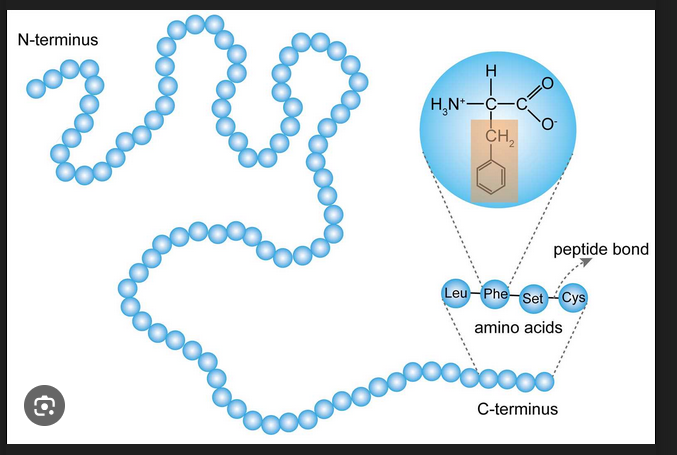
\includegraphics[width=0.8 \textwidth]{protein.png}
			\caption{Primary structure of a protein}
			\href{https://www.creative-biostructure.com/levels-of-protein-structure.htm?srsltid=AfmBOopCotOwaj1i5c8CxJtbmB6Nv53b5btbOnjC4BGknPWKFYbO-UkX}{Source}
			\label{fig:protein}
		\end{figure}
	\end{frame}
	\begin{frame}
		\frametitle{A bit about the research of proteins}
		\begin{itemize}
			\item Probably hundreds of papers that get publish every year - some of them revolutionary, some of them useless
			\item The reasons are various: curiosity, need to cure illnesses, a must to find vaccines
			\item Limitations: time consuming procedures, manual operations, error prone processes, replicability issues, specialized knowledge
		\end{itemize}
	\end{frame}
	\begin{frame}
		\frametitle{What is this paper about?}
		\begin{itemize}
			\item Generalized platform that make use of the cross edge technologies we have nowadays: LLMs, electricity, machine learning pipelines, existing lab systems
			\item End goals: biologist friendly, costs and time efficient, fully automated, easily configurable or extended
			\item Q: What does the system do? A: In short, the system represents a biofoundry platform that respects the DBTL flow: design, build, test and learn
		\end{itemize}
	\end{frame}
	\begin{frame}
		\frametitle{How does this system work?}
		\begin{itemize}
			\item Design the proteins using a special LLM by applying single amino-acid mutations
			\item Checks their properties using a specialized automation platform for lab experiments, called iBioFAB
			\item Sequence a small number of mutants to observe their characteristics and compose the train dataset for the model
			\item Train a supervised ML model based on the gathered data from the sequenced mutated proteins
			\item Finally, the trained model will then guide that special LLM in its decisions regarding what mutations to make - and thus the cycle repeats
		\end{itemize}
	\end{frame}
	\begin{frame}
		\frametitle{Design}
		\begin{itemize}
			\item Protein-LLM called ESM-2, which is actually a transformer model trained on global protein sequences that predicts the likelihood of amino acids
			\item EVmutation - an epistasis model
			\item Supervised low-N regression model trained on the previous rounds outcomes
			\item EVcouplings: a statistical model for scoring the impact of amino-acids substitutions
			\item LLM UI: LLM-created UI leveraging OpenAI’s assistant API with customized functions
			\item Examples of prompts: "help me improve phytase" or "design the initial library for AtHMT"
		\end{itemize}
	\end{frame}
	\begin{frame}
		\frametitle{Epistasis}
		\begin{figure}[h]
			\centering
			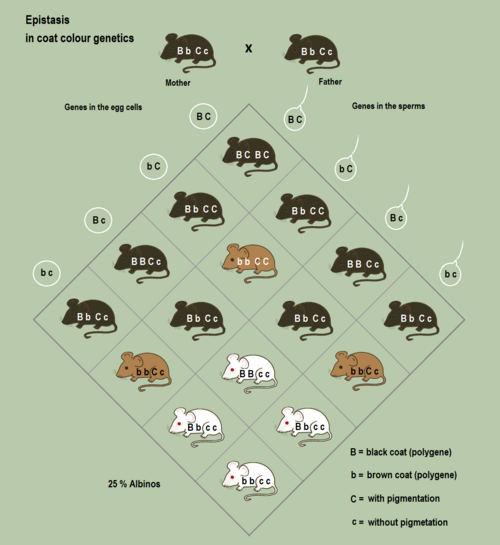
\includegraphics[width=0.8 \textwidth]{epistasis.png}
			\caption{Example of an Epistasis Model}
			\href{https://en.wikipedia.org/wiki/Epistasis}{Source}
			\label{fig:epistasis}
		\end{figure}
	\end{frame}
	\begin{frame}
		\frametitle{Build}
		\begin{itemize}
			\item iBioFAB: a laboratory automation platform that combines various instruments for robust and continuous experimentation, like creating and mutating proteins
			\item Design new protein sequences (natural or engineered)
			\item Express the proteins in cells (like bacteria or yeast)
			\item Test their structure, function, and performance
			\item Iteratively improve them using data
			\item Problem: To sequence and verify the mutated candidates you have to apply site-directed mutagenesis (SDM)
			\item Solution: Only a small percent from the set of candidates are sequenced and measured to generate the desired dataset
			\item Modular system
		\end{itemize}
	\end{frame}
	\begin{frame}
		\frametitle{iBioFab}
		\begin{figure}[h]
			\centering
			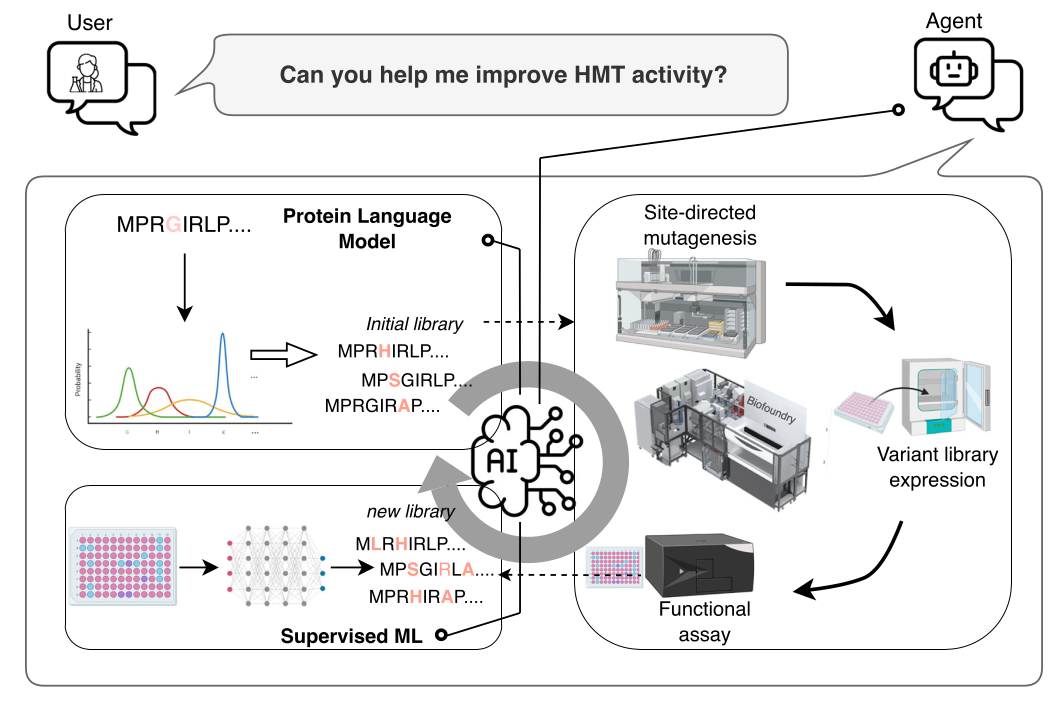
\includegraphics[width=0.8 \textwidth]{ibiofab.png}
			\caption{Procedures inside iBioFAB}
			\href{https://doi.org/10.1038/s41467-025-61209-y}{Source}
			\label{fig:ibiofab}
		\end{figure}
	\end{frame}
	\begin{frame}
		\frametitle{Test and Learn}
		\begin{itemize}
			\item iBioFAB analyze the synthesized variants and puts them under multiple tests to gather enough data
			\item the data gathered from the previous step produced on the last step is used to train the supervised model to further improve the performance of the LLM
		\end{itemize}
	\end{frame}
	\begin{frame}
		\frametitle{Examples and Results - 1}
		\begin{itemize}
			\item Goal: improve enzymatic properties of 2 proteins			
			\item AtHMT protein - ethyltransferase activity which offers potential for synthesizing S-adenosyl-L-methionine (SAM) analogs, which are essential for biocatalytic alkylation, a process with crucial biological applications
			\item YmPhytase - broaden the range of pH when it's active
			\item Phytase can hydrolyze phytic acid, the main storage form of phosphate in plant tissues that is indigestible by most animals, and release inorganic phosphate, an important nutrient
		\end{itemize}
	\end{frame}
	\begin{frame}
		\frametitle{Examples and Results - 2}
		\begin{itemize}
			\item After 4 rounds, the best identified AtHMT variant showed an 16-fold improvement in ethyltransferase activity; another AtHMT variant showed an 90-fold increase in preference for ethyl-iodide over methyl-iodide.
			\item For YmPhytase, one variant from the fourth round exhibited a 26.3-fold improvement in specific activity over wtPhy at pH 6.6. Another variant performed remarkably well at both pH 5.6 and 6.6, exhibiting 25.8- and 19.8-fold improvements in specific activity compared to wtPhy, respectively. 
		\end{itemize}
	\end{frame}
	\begin{frame}
		\frametitle{Results Graphics}
		\begin{figure}[h]
			\centering
			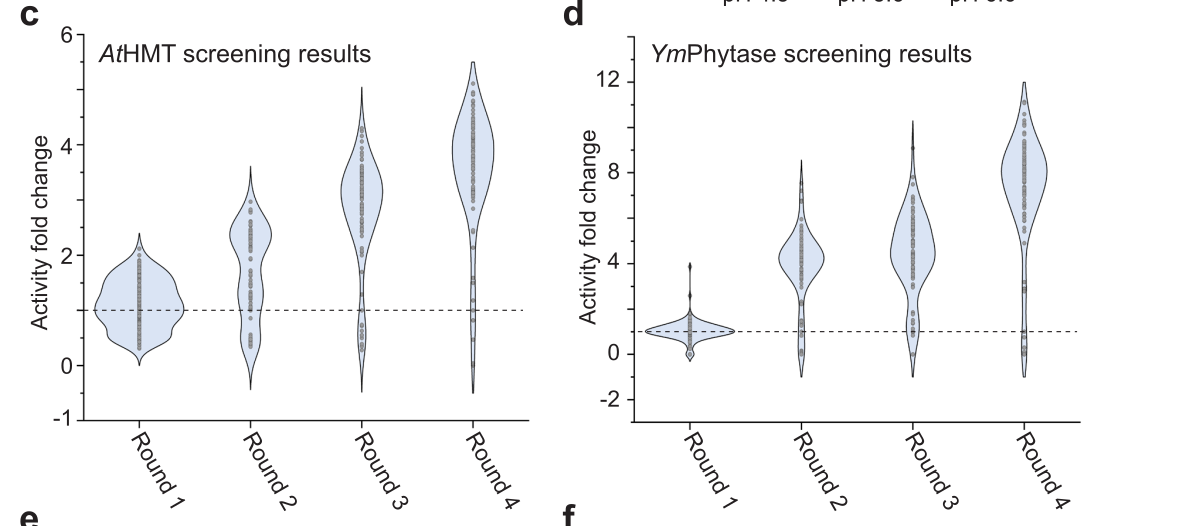
\includegraphics[width=0.8 \textwidth]{results.png}
			\caption{(c) The fold change in HMT ethyl-transferase activity with respect to the wild type is shown in a violin plot for four rounds of crude lysate screening (n >= 3 biological replicates). (d) The fold change in phytase activity with respect to the wild type is shown in a violin plot for four rounds of crude lysate screening (n >= 3 biological replicates)}
			\href{https://doi.org/10.1038/s41467-025-61209-y}{Source}
			\label{fig:results}
		\end{figure}
	\end{frame}
	\begin{frame}
		\frametitle{Limitations}
		\begin{itemize}
			\item ESM-2 may not be suitable for all proteins
			\item The supervised low-N model used for iterative predictions showed relatively weak correlation with experimental results
			\item Recycling of mutagenesis prevents parallelization
			\item High throughput proteins
			\item Toxic proteins
		\end{itemize}
	\end{frame}
	\begin{frame}
		\frametitle{Cell Free Protein Synthesis}
		\begin{itemize}
			\item Can be used as a first test
			\item Initial data set optimization
			\item Better understanding of how certain DNA sequences create different toxic proteins
		\end{itemize}
	\end{frame}
	\begin{frame}[c,plain]
		\centering
		\Huge ¿Teneis alguna pregunta?
	\end{frame}
\end{document}


